\section{Creating Language Definition in MPS}
\label{sect:LANGDEF}

The proposed INGRID method accepts grammars in the ANTLR v4 notation~\cite{ref:ANTLRBOOK} as input.
All widely used programming languages have their syntax defined using this notation~\footnote{https://github.com/antlr/grammars-v4}.
Unlike some of the related projects, we did not extend the notation with any custom features, and we also did not create an MPS language for the ANTLR notation.

The process of MPS language construction, as performed by INGRID, consists of four phases --- the first is parsing of the input grammar, which is followed by definition of the essential aspects of the language (Structure, Editor, and TextGen).
Each of the phases 2-4 is exclusively and fully responsible for one aspect.

INGRID is currently able to create (i) a full Structure aspect for each element (type of an AST node) of the given language, (ii) a very basic Editor, and (iii) a basic TextGen aspect.
Therefore, the resulting MPS language typically still has to be adjusted manually to improve its usability, and the human users must also define the remaining aspects not yet supported by INGRID.

Our approach differs from the related projects (Section~\ref{sect:RELATED}) especially in the level of automation. It also has much better support for the definition of Editor and TextGen.

\subsection{Running Example}

We will describe the INGRID method using the example of a simplified XML language that is defined in Figure~\ref{fig:SIMPLEXML}.
The \emph{SimpleXML} language is small but complex enough to be used for illustration of the main challenges and behavior of the proposed algorithms.

\begin{figure*}[ht]
\centering
\begin{framed}
\begin{alltt}
\textbf{grammar} \textit{SimpleXML};
\antlrparserrule{document}  : \antlrparserrule{prolog}? \antlrparserrule{comment}? \antlrparserrule{element} ;
\antlrparserrule{prolog}    : \antlrliteral{<?xml } \antlrparserrule{attrib}* \antlrliteral{?>} ;
\antlrparserrule{comment}   : \antlrliteral{<!--} \antlrlexerrule{TEXT} \antlrliteral{-->} ;
\antlrparserrule{element}   : \antlrliteral{<} \antlrlexerrule{Name} \antlrparserrule{attrib}* \antlrliteral{>} \antlrparserrule{content}* \antlrliteral{</} \antlrlexerrule{Name} \antlrliteral{>} | \antlrliteral{<} \antlrlexerrule{Name} \antlrparserrule{attrib}* \antlrliteral{/>} ;
\antlrparserrule{attrib}    : \antlrlexerrule{Name} \antlrliteral{="} \antlrlexerrule{TEXT} \antlrliteral{"} ;
\antlrparserrule{content}   : \antlrlexerrule{TEXT} | \antlrparserrule{element} | \antlrparserrule{comment} | \antlrlexerrule{CDATA} ;
\antlrlexerrule{Name}      : \antlrlexerrule{NameStartChar} \antlrlexerrule{NameChar}* ;
\textbf{fragment}
\antlrlexerrule{DIGIT}     : \antlrregex{[0-9]} ;
\textbf{fragment}
\antlrlexerrule{NameChar}  : \antlrlexerrule{NameStartChar} | \antlrliteral{-} | \antlrliteral{\_} | \antlrliteral{.} | \antlrlexerrule{DIGIT} ;
\textbf{fragment}
\antlrlexerrule{NameStartChar} : \antlrregex{[:a-zA-Z]} ;
\antlrlexerrule{TEXT}      : \antlrregex{~[<"]*} ;
\antlrlexerrule{CDATA}     : \antlrliteral{<![CDATA[} \antlrregex{.*?} \antlrliteral{]]>} ;
\end{alltt}
\end{framed}
\caption{Grammar of the SimpleXML language in the ANTLR v4 notation}
\label{fig:SIMPLEXML}
\end{figure*}

The grammar of SimpleXML contains elements of the kinds that are listed below.
Each color in Figure~\ref{fig:SIMPLEXML} corresponds to a different kind in a way that is indicated by the list item headers.
\begin{itemize}
	\item \textbf{ANTLR v4 keywords} are required by the notation.
	\item \antlrparserrule{\textbf{Parser rules}} describe the structure of a language.
		Alternatives on the right side of a rule are separated by the pipe character ($|$).
	\item \antlrlexerrule{\textbf{Lexer rules}} describe terminal symbols that the parser matches against the input string.
		A terminal symbol can be encoded as a string value or using a regular expression.
		The \textbf{fragment} keyword states that the lexer rule just brings more clarity into the notation but it is not visible in the parser output.
	\item \antlrliteralnoap{\textbf{String literals}}, always written inside of a pair of single quote marks, also represent terminal symbols, but by exact match to a string constant.
	\item \antlrregex{\textbf{Regular expressions}} describe string tokens to be matched against regular expressions with a special ANTLR v4 regex notation\footnote{https://github.com/antlr/antlr4/blob/master/doc/lexer-rules.md}.
\end{itemize}
Elements on the right side of a rule can be annotated with standard EBNF operators (\code{?}, \code{+}, \code{*}) that specify the allowed number of occurrences.

\subsection{Phase 1: Parsing Input Grammar}

The first phase in the process of MPS language construction is parsing of the input grammar that is defined using the ANTLR v4 notation.
An output of this phase is an AST representing the grammar.
Nodes of the AST correspond to rules and other grammar elements.

Nevertheless, the full AST, which comes out of the automatically generated parser, is quite complex and contains information not relevant for the INGRID algorithm.
In order to get a simple representation that is easy process by the later phases and keeps only information necessary for the construction of MPS languages, several steps of post-processing of the AST have to be performed in this phase.

A simplified tree of objects is derived from the AST in two passes over the grammar.
The result of the first pass is a tree where each node contains names of other referenced rules in the form of strings.
In the second pass, the whole tree is traversed and all the references are resolved to have a form of real pointers to other rule objects.

The representation of lexer rules (tokens) in the AST has to be simplified too.
Note that, in the ANTLR notation, lexer rules can be built from alternatives just like the parser rules --- see, for example, the lexer rule \antlrlexerrule{Name} from our SimpleXML language (Figure~\ref{fig:SIMPLEXML}).
For each lexer rule, the parser produces a tree that captures the structure of the rule.
However, the lexer rules are, in fact, just regular expressions used to recognize tokens in the input string.

Every tree that represents a lexer rule is flattened into the equivalent regular expression by the recursive algorithm specified in Figure~\ref{fig:ALGFLATTEN}.
A distinct sequence is created from the elements of each alternative, and then all those sequences are joined by the alternation operator \code{$|$} to form a regular expression.

\begin{figure}[ht]
\centering
\begin{framed}
\begin{alltt}
Flatten(\textit{R}):
  \textit{T} = empty list
  \textbf{for each} alternative \textit{A} \textbf{in} rule \textit{R}:
    \textit{R} = \antlrap\antlrap
    \textbf{for each} element \textit{E} \textbf{of} \textit{A}:
      \textbf{if} \textit{E} is not yet flattened \textbf{then}:
        Flatten(\textit{E})
      \textit{R}.append(\textit{E})
      \textit{R}.append(\textit{E}.operator)
    \textit{T}.add(\textit{R})
  build string S from elements of \textit{T}:
    \textit{S} = \(t\sb{1}\) | \(t\sb{2}\) | \(\ldots\) | \(t\sb{n}\)
  \textbf{return} \textit{S}
\end{alltt}
\end{framed}
\caption{Flattening algorithm}
\label{fig:ALGFLATTEN}
\end{figure}

The output of \texttt{Flatten(Name)}, i.e. application of the algorithm to the \antlrlexerrule{Name} rule, is this regular expression:

\begin{center}
  \texttt{[:a-zA-Z]([:a-zA-Z]|\textbackslash-|{\_}|\textbackslash.|[0-9])*}
\end{center}
It defines the syntactically valid identifiers of elements and attributes in SimpleXML.
Each identifier must begin with a letter, followed by any combination of letters, digits, underscore, dash, or a dot.

\subsection{Phase 2: Structure}

In the next phase, the complete structure of the MPS language is automatically generated from the AST that represents syntax of the input language.
Elements of the Structure aspect are derived from the AST nodes, and then linked appropriately.
Therefore, structure of the MPS language is usually similar to the original ANTLR grammar.

When designing the process for translating AST nodes (i.e., grammar rules) into the MPS language structure, we faced several challenges.
The main challenge related to the structure, as we already mentioned in the introduction, is that a grammar typically contains rules that do not directly correspond to programming language constructs.
Such rules exist at the intermediate layers of a syntax hierarchy.
Their main purpose is to enable easier understanding and maintenance of the grammar by humans.
However, presence of the intermediate layers significantly complicates usage of the given language in MPS, and the layers are actually not necessary for construction of an MPS language.
We show examples illustrating this problem, which we call a \emph{layer problem}, later in the subsection where we describe our solution.

As a part of the INGRID method, we have designed an approach to eliminate the unnecessary layers during construction of the Structure aspect --- we call it the \emph{shortcut} approach (Section~\ref{sect:SHORTCUT}).
However, before focusing on the intermediate layers and the shortcut approach, we describe the basic principles of translation from the AST into the language structure.

Each concept of the language (i.e., every AST node) is represented by an object that may have a parent, some children, and properties of any data type.
In addition, the object may implement any number of interfaces, and it may also contain references to objects representing other AST nodes.
The parent-child relationships between objects that make the Structure aspect are derived from rules of the grammar (i.e., from the structure of the AST).
For each rule, the object corresponding to the left-hand side is in the parent-child relationships with sets of objects that represent language elements referenced by the right-hand side.
If a rule has multiple alternatives, then a distinct object (MPS concept) has to be created in the structure for each alternative.
The name of a concept (object) in MPS is composed from (1) the name of the AST node, which is equivalent to the string encoding of the left-hand side of the corresponding rule, and (2) the number indicating the position of the respective alternative on the right-hand side of the rule.

\begin{figure}[ht]
\centering
\begin{alltt}
\small
\mpsstkeyword{concept} Element\_1 \mpsstkeyword{extends} BaseConcept
        \mpsstkeyword{implements} IContent, IElement

  \mpsstkeyword{instance can be root:} false
  \mpsstkeyword{alias:} \mpsstalias{< > </ >}
  \mpsstkeyword{short description:} \mpsstalias{Element}

  \mpsstkeyword{properties:}
  \mpsstproperty{Name\_1} : Name
  \mpsstproperty{Name\_2} : Name
  
  \mpsstkeyword{children:}
  \mpsstproperty{Attribute\_1} : Attribute[\mpsstcardinality{0..n}]
  \mpsstproperty{Content\_2}   : IContent[\mpsstcardinality{0..n}]
\end{alltt}
\caption{Structure aspect of the \code{Element{\_}1} concept}
\label{fig:ELEMENTSTRUCT}
\end{figure}

Consider the parser rule \antlrparserrule{element} from the grammar in Figure~\ref{fig:SIMPLEXML}.
Its first alternative represents the full XML element with content.
Figure~\ref{fig:ELEMENTSTRUCT} shows the Structure aspect for the MPS concept (object) named \code{Element{\_}1} that corresponds to the alternative.
The object contains two properties, one for each reference to the lexer rule \antlrlexerrule{Name}.
Values of these properties should be restricted using the regular expression that corresponds to the \antlrlexerrule{Name} rule, but this is left to the human user.
String literals, such as the keyword \textbf{for}, are omitted because they will be defined only in the Editor aspect for this concept.

References to other parser rules are captured by pointers to child objects.
The types of child objects, such as \code{IContent} in the \code{Element{\_}1} concept, are determined as follows.
Consider the \antlrparserrule{content} rule from the SimpleXML language.
We show just the relevant fragment of the grammar again in Figure~\ref{fig:CONTENTRULE}.
An object corresponding to any one of the four alternatives could be the actual value anywhere the \antlrparserrule{content} rule is referenced.

\begin{figure}[ht]
\centering
\begin{alltt}
\small
\antlrparserrule{content} : \antlrlexerrule{TEXT} | \antlrparserrule{element} | \antlrparserrule{comment} | \antlrlexerrule{CDATA} ;
\end{alltt}
\caption{Parser rule \antlrparserrule{content}}
\label{fig:CONTENTRULE}
\end{figure}

Our solution is to use interface concepts.
For each rule with more than one alternative on the right side, i.e. for each AST node with more than one child, first an interface concept is defined in the MPS language structure, and then one object that implements the given interface is created for each alternative.
The resulting fragment of the language structure looks like the one in Figure~\ref{fig:ICONTENTITF}.
It contains one interface \mpsinterface{IContent} that is implemented by four object concepts \mpsconcept{Content{\_}1}, $\ldots$, \mpsconcept{Content{\_}4}.

\begin{figure}[ht]
\centering
\begin{alltt}
\small
\mpsinterface{IContent} : \mpsconcept{Content{\_}1} | \mpsconcept{Content{\_}2} |
           \mpsconcept{Content{\_}3} | \mpsconcept{Content{\_}4}
\end{alltt}
\caption{MPS interface \code{IContent} and the types of implementing objects}
\label{fig:ICONTENTITF}
\end{figure}

Now we can illustrate the layer problem on the behavior of auto-completion in MPS.
Suppose that a user is creating a new document in the SimpleXML language, just inserted a fresh node of the type \mpsconcept{Element{\_1}} (see above), and would like to insert another nested XML element inside.
The auto-completion mechanism of MPS offers four options that are displayed in the left part of Figure~\ref{fig:LAYERPROBLEM}.
Each option represents one of the MPS concepts that implement the interface \mpsinterface{IContent}, and therefore also one alternative of the \antlrparserrule{content} rule.

\begin{figure*}[ht]
	\centering
	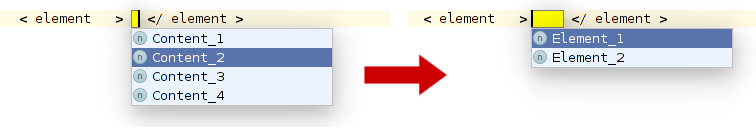
\includegraphics[scale=0.5]{./images/layer_problem.png}
	\caption{Layer problem in auto-completion}
	\label{fig:LAYERPROBLEM}
\end{figure*}

However, in order to correctly insert another nested element, a user has to perform two steps:
\begin{enumerate}
	\item Insert an object (node) of the type \mpsconcept{Content{\_}2} inside the \mpsconcept{Element{\_}1} node. The \mpsconcept{Content{\_}2} object has only a single child node of the interface type \mpsinterface{IElement}.
	\item Then, the user must trigger the auto-complete again and insert either an \mpsconcept{Element{\_}1} node or an \mpsconcept{Element{\_}2} node into the \mpsconcept{Content{\_}2} node. See the right part of Figure~\ref{fig:LAYERPROBLEM}.
\end{enumerate}
The main difficulty here is that, in the first step, the user has to (i) either correctly guess what option offered by the auto-complete menu to select, or (2) to remember the order of alternatives in the grammar rule.

Similarly, if the user would like to replace a nested \mpsconcept{Element{\_}1} node with, for example, an XML comment (represented by the \mpsconcept{Comment} node), then both intermediary layers have to be deleted before she gets back to the original selection among the concepts \mpsconcept{Content{\_}1}, $\ldots$, \mpsconcept{Content{\_}4}.

Intermediary layers have no visual appearance, and therefore it is very difficult for users to see what is actually happening and they may get confused very easily.
The layer problem is addressed by the shortcut approach, which we describe in the next subsection.

\subsubsection{The Shortcut Approach}
\label{sect:SHORTCUT}

The key idea of this approach is to skip all the intermediary layers (nodes) in the syntax tree and consider just the leaf nodes, e.g., to be directly offered to the user through the auto-completion menu.
Specifically, the \antlrparserrule{content} rule from the SimpleXML grammar, which is given in Figure~\ref{fig:CONTENTRULE} together with rules that determine the relevant fragment of the syntax hierarchy, expands ultimately into the leaf nodes that are highlighted using the bold font in Figure~\ref{fig:CONTENTEXPAND}.

\begin{figure*}[ht]
\centering
\begin{framed}
\begin{alltt}
  \antlrparserrule{content} : \antlrlexerrule{TEXT} | \antlrparserrule{element} | \antlrparserrule{comment} | \antlrlexerrule{CDATA} ;
  \antlrparserrule{element} : \antlrliteral{<} \antlrlexerrule{Name} \antlrparserrule{attrib}* \antlrliteral{>} \antlrparserrule{content}* \antlrliteral{</} \antlrlexerrule{Name} \antlrliteral{>} | \antlrliteral{<} \antlrlexerrule{Name} \antlrparserrule{attrib}* \antlrliteral{/>} ;
  \antlrparserrule{comment} : \antlrliteral{<!--} \antlrlexerrule{TEXT} \antlrliteral{-->} ;
\end{alltt}
\end{framed}
\caption{The parser rule \antlrparserrule{content} with other rules that determine the relevant fragment of the syntax hierarchy}
\label{fig:CONTENTRULE}
\end{figure*}

\begin{figure}[ht]
\begin{framed}
\textbf{Content{\_}1} (TEXT) \\
\ \ \ Content{\_}2 $\rightarrow$ \textbf{Element{\_}1} \\
\ \ \ Content{\_}2 $\rightarrow$ \textbf{Element{\_}2} \\
\ \ \ Content{\_}3 $\rightarrow$ \textbf{Comment} \\
\ \ \ \textbf{Content{\_}4} (CDATA)
\end{framed}
\caption{Leaf nodes of the parser tree fragment that has the \antlrparserrule{content} rule as its root}
\label{fig:CONTENTEXPAND}
\end{figure}

For the input that consists of a particular AST node $N$ and the grammar rule $R$ that expands $N$, the procedure implementing the shortcut approach systematically traverses the parser tree (AST) built in the earlier phases in order to identify each AST node that may appear at the end of some derivation chain starting by the rule $R$ from the node $N$.
Such nodes cannot expand further based on any rule in the grammar, and for that reason we call them \emph{end nodes}.

\begin{figure*}[ht]
\begin{framed}
\begin{alltt}
 1 FindAllPathsToEndNodes(\textit{R}):
 2   \textit{CurPath} = empty list of rules and nodes
 3   \textbf{return} FindPaths(\textit{R}, \textit{CurPath})
 4
 5 FindPaths(\textit{R}, \textit{CurPath}):
 6  \textit{Paths} = empty list
 7  \textbf{for each} alternative \textit{A} \textbf{in} rule \textit{R}:
 8    \textit{NewCurPath} = Clone(\textit{CurPath})
 9    \textbf{if} \textit{A} contains only a single element \textit{E}:
10      \textit{NewCurPath}.Add(\(N\sb{E}\)) \textbf{where} \(N\sb{E}\) is the node representing \textit{E}
11      \textit{P} = FindPaths(\(R\sb{E}\), \textit{NewCurPath}) \textbf{where} \(R\sb{E}\) is the rule that expands \textit{E}
12      \textit{Paths} = Merge(\textit{Paths}, \textit{P})
13    \textbf{else}:
14      \textit{NewCurPath}.Add(\textit{R})
15      \textit{NewCurPath}.Add(\(N\sb{A}\)) \textbf{where} \(N\sb{A}\) is the node representing \textit{A}
16      \textit{Paths}.Add(\textit{NewCurPath})
17  \textbf{return} \textit{Paths}
\end{alltt}
\end{framed}
\caption{Algorithm to find all paths to end nodes for a parser rule}
\label{fig:SHORTCUTALG}
\end{figure*}

Figure~\ref{fig:SHORTCUTALG} shows the algorithm that finds all paths to some end node from a given parser rule $R$.
The algorithm is based on recursive traversal of the parser tree.
At each level of recursion, it gathers all paths that lead from the current parser rule $R$ to some end node through its alternatives (line~7).
Two cases may occur:
\begin{itemize}
	\item When a particular alternative $A$ of the rule $R$ contains only a single element $E$, and the element is a reference to another parser rule (line 9), the alternative $A$ is an intermediary layer that can be transparently hidden from the user of the MPS language.
		  A run of the algorithm continues, at line 11, by recursively processing alternatives of the rule corresponding to $E$, which lies at the next level of the parser tree.
	\item Otherwise, an end node of a derivation chain was found and the recursion stops (lines 13-16).
\end{itemize}
By appending the node corresponding to the current alternative (lines 10 and 15) and the rule that leads to the alternative (line 14), the algorithm creates a full path that contains the target end node as the last element of the chain.

We use the name \emph{shortcut approach} for this algorithm, because the paths collected by the algorithm provide shortcuts from the given rule to end nodes, by the virtue of hiding all intermediary layers.
For example, the result of this algorithm for the \antlrparserrule{content} rule (Figure~\ref{fig:CONTENTRULE}) is the list of five items already shown in Figure~\ref{fig:CONTENTEXPAND}.

The primary use case for shortcuts is to generate options for the auto-completion menus, such that only the end nodes are offered.
Shortcuts have to be considered not only when nodes are inserted, but also when they are deleted.
In each case, the whole chain including possibly multiple intermediary AST nodes (up to the end node) must be added, respectively deleted.
When the user wants to delete some end node from the AST of a program or document written in the MPS language, the effect of an insertion must be fully reversed.

\subsection{Phase 3: Editor}

Having the complete structure of the new MPS language, the next phase is to define the visual representation of all concepts (AST nodes) in the projectional editor.
As we said in Section~\ref{sect:MPS}, MPS uses a cellular system that enables the language developer to arrange the children and properties of an AST node in a table-like manner.
Cells of different types are supported by MPS --- for storing property values, references to child nodes, and keywords (string literals), and also cells that influence layout (e.g., indentation).
The specific goal of this phase is to create the Editor aspect for each language concept (element), such that all attributes of the concept --- name, properties, children --- are projected using the respective cell types.

The main problem that we had to address is the absence of information about the code layout and whitespace in the ANTLR grammar of an input language.
Rules forming the grammar only tell what the syntax tree looks like and how the program code is decomposed into AST nodes.
Here we present a solution that is only partially automated for reasons explained below.

We experimented with several heuristics to derive a useful code layout, but all of them produced rather suboptimal results.
However, we observed that the most tedious and error-prone step in the manual definition of the Editor aspect is the creation of cells for all literals (keywords), properties, children, and other fields of a given concept that should appear in its visual representation.
This step can be very easily automated.

Our solution that we implemented in the current version of the INGRID method is to create all the cells and place them in a single row.
The resulting basic layout is illustrated on the example of the \mpsconcept{Element{\_}1} concept in the upper left corner of Figure~\ref{fig:EDITORADJUST}.
Further adjustments of the layout, such as indentation and line breaks, can be done very efficiently in the MPS IDE.
The bottom right part of Figure~\ref{fig:EDITORADJUST} shows a fully customized layout for the \mpsconcept{Element{\_}1} concept.

\begin{figure*}[ht]
	\centering
	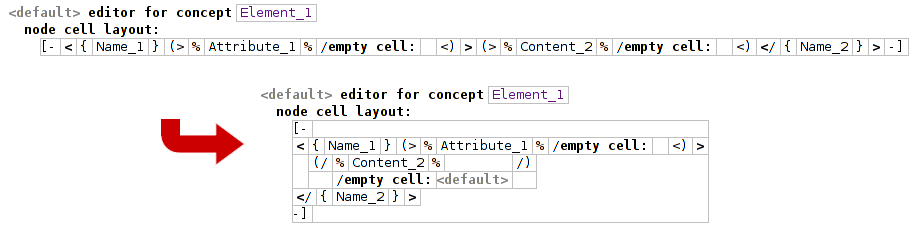
\includegraphics[scale=0.55]{./images/editor_adjustment.png}
	\caption{Editor aspect of the \mpsconcept{Element{\_}1} concept}
	\label{fig:EDITORADJUST}
\end{figure*}

Based on our experience, it takes a very short time to manually adjust the layout into a form much better than any fully automated heuristic could achieve.
We expect that a typical user of the INGRID method will be able to use the projectional editor in MPS quite efficiently.
More details are provided in Section~\ref{sect:EVAL}, including our experience with several mainstream programming languages.

We have found that the combination of two steps, (1) automated placing of cells into a single row and (2) subsequent manual adjustment of the layout, is a very fast and efficient way of creating a nice code layout.
Nevertheless, we plan to work on a more automated approach to the definition of Editor aspects in the future, probably using some techniques of machine learning.
The key idea would be to derive the code layout from a set of valid input source files.
We believe that the user would have to adjust the editor manually a little bit even in this case, because the results of a machine learning-based approach would not be perfect.

\subsection{Phase 4: Text Generation}

The purpose of the last phase of the MPS language construction is to generate the TextGen aspect for each concept.
We use the \mpsconcept{Element{\_}1} concept again for illustration.
Figure~\ref{fig:TEXTGENBASIC} shows a very basic example of BaseLanguage code that can be used as its TextGen aspect.
The code appends all literals, properties, and children of \mpsconcept{Element{\_}1} to the output buffer, and does that in the same order as they appear in the corresponding grammar rule.

\begin{figure}[ht]
\begin{alltt}
\small
\mpstgkeyword{text gen component for concept} \mpstgtarget{Element{\_}1} \{
  \mpstgparam{(context, buffer, node)->void} \{
    \mpstgaction{append} \{\mpstgliteral{<}\};
    \mpstgaction{append} \$\{\mpstgparam{node}.\mpstgnodeprop{\textit{Name}}{\_}\textit{1}\};
    \mpstgaction{append} \{\ \};
    \mpstgaction{append} \$list\{\mpstgparam{node}.\mpstgnodeprop{\textit{Attribute}}{\_}\textit{1}\};
    \mpstgaction{append} \{\mpstgliteral{>}\};
    \mpstgaction{append} \$list\{\mpstgparam{node}.\mpstgnodeprop{\textit{Content}}{\_}\textit{2}\};
    \mpstgaction{append} \{\mpstgliteral{</}\};
    \mpstgaction{append} \$\{\mpstgparam{node}.\mpstgnodeprop{\textit{Name}}{\_}\textit{2}\};
    \mpstgaction{append} \{\mpstgliteral{>}\};
  \}
\}
\end{alltt}
\caption{Basic TextGen aspect for the \mpsconcept{Element{\_}1} concept}
\label{fig:TEXTGENBASIC}
\end{figure}

Like in the case of a projectional editor, the main challenge associated with TextGen is to produce valid code with a reasonable layout.
An implementation of the TextGen aspect must determine properly where to put line breaks, indentation, and other whitespace characters.
For example, in the case of the concept representing an XML element, there must be a space between the element's name and the first attribute, while it is not required between the opening bracket \antlrliteral{\textless} and the name (Figure~\ref{fig:TEXTGENBASIC}).

Our INGRID method targets mostly text-based languages, for whose concepts the visual representation in a projectional editor must be almost equivalent to their plain-text representation.
An obvious choice would therefore be to use the same approach for Editor and TextGen.
Nevertheless, since the Editor aspect has to be adjusted manually, we decided to use a different approach for TextGen.
We designed a procedure based on a simple fully automated heuristic that provides surprisingly good results.

The procedure creates the TextGen aspect for a given language concept (AST node) in two steps.
First, it generates a basic variant that inserts spaces in between every two tokens of the textual representation of the concept.
In the second step, which is the core of our heuristic, spaces are eliminated from places where they are not really needed.
The main criterion is whether the generated plain-text output can be safely processed by a parser of the original language (using the ANTLR grammar).
We discuss all the cases here:
\begin{itemize}
	\item When there is a non-alphabetical literal that is used as a token in the grammar, and that might get recognized by the parser without the need for whitespace separators around it, then we can omit the spaces. An example of such literal is '\textless' in SimpleXML.
	\item In the case of an arbitrary string, the whitespace may be omitted when the adjacent literal ends, respectively begins, with a non-alphabetical character.
		This applies especially to the values of properties defined in Structure aspects, such as the name of an XML element.
		Based on this heuristic, redundant spaces inside of quotes will be eliminated, as well as spaces next to semicolons and around brackets.
		On the other hand, it will distinguish language keywords (e.g., \code{function}, \code{var}, \code{in}) from other literals by preserving the space character in between them.
	\item Spaces can be safely omitted also when specific optional child nodes are not present, and in the case of empty lists of child nodes, so that whitespace does not accumulate.
\end{itemize}
A space must be alway inserted when two child nodes are next to each other.
Elements of a sequence of child nodes are separated with space or a line break.

\begin{figure}[ht]
\begin{alltt}
\small
\mpstgkeyword{text gen component for concept} \mpstgtarget{Element{\_}1} \{
  \mpstgparam{(context, buffer, node)->void} \{
    \mpstgaction{append} \{\mpstgliteral{<}\};
    \mpstgkeyword{if} (\mpstgparam{node}.\mpstgnodeprop{\textit{Name}}{\_}\textit{1}.\textbf{isNotEmpty}) \{
      \mpstgaction{append} \$\{\mpstgparam{node}.\mpstgnodeprop{\textit{Name}}{\_}\textit{1}\};
    \}
    \mpstgkeyword{if} (\mpstgparam{node}.\mpstgnodeprop{\textit{Attribute}}{\_}\textit{1}.\textbf{size} > 0) \{
      \mpstgaction{append} \{\ \};
      \mpstgaction{append} \$list\{\mpstgparam{node}.\mpstgnodeprop{\textit{Attribute}}{\_}\textit{1} with  \};
    \}
    \mpstgaction{append} \{\mpstgliteral{>}\};
    \mpstgkeyword{if} (\mpstgparam{node}.\mpstgnodeprop{\textit{Content}}{\_}\textit{2}.\textbf{size} > 0) \{
      \mpstgaction{append} \$list\{\mpstgparam{node}.\mpstgnodeprop{\textit{Content}}{\_}\textit{2} with  \};
    \}
    \mpstgaction{append} \{\mpstgliteral{</}\};
    \mpstgkeyword{if} (\mpstgparam{node}.\mpstgnodeprop{\textit{Name}}{\_}\textit{2}.\textbf{isNotEmpty}) \{
      \mpstgaction{append} \$\{\mpstgparam{node}.\mpstgnodeprop{\textit{Name}}{\_}\textit{2}\};
    \}
    \mpstgaction{append} \{\mpstgliteral{>}\};
  \}
\}
\end{alltt}
\caption{Full TextGen aspect for the \mpsconcept{Element{\_}1} concept}
\label{fig:TEXTGENFINAL}
\end{figure}

\begin{figure}[ht]
\begin{alltt}
\small
\mpstgkeyword{if} (\mpstgparam{node}.\mpstgnodeprop{\textit{Content}}{\_}\textit{2}.\textbf{size} > 0) \{
  \mpstgaction{append} \textcolor{Blue}{\textbf{\textbackslash{}n;}}
  \mpstgaction{indent buffer;}
  \mpstgkeyword{with indent} \{
    \mpstgaction{append} \$list\{\mpstgparam{node}.\mpstgnodeprop{\textit{Content}}{\_}\textit{2} with  \};
  \}
  \mpstgaction{append} \textcolor{Blue}{\textbf{\textbackslash{}n;}}
\} 
\end{alltt}
\caption{Fragment of the TextGen aspect of \mpsconcept{Element{\_}1} with adjusted indentation}
\label{fig:TEXTGENADJUSTED}
\end{figure}

Figure~\ref{fig:TEXTGENFINAL} contains the complete, automatically generated, TextGen aspect for the \mpsconcept{Element{\_}1} concept, which represents the full SimpleXML element.
Such code may be adjusted manually very easily in order to produce nicely indented XML documents.
We only need to wrap the \mpsconcept{Content{\_}2} child node with indentation and change the sequence separator to a new line character.
A fragment of the resulting adjusted aspect (code) is in Figure~\ref{fig:TEXTGENADJUSTED}.





% TODO continue from here



\subsection{Remarks about Grammars}

As we have already shown in previous sections, it is very easy to write a grammar in a way that will cause problems during import into MPS (or once it is imported).
Problems might occur during the creation of any aspect.
Here we will look at some general problems/issues that grammar import poses (might pose).
We will talk about these problems with respect to the challenges/obstacles we tried to overcome and which we described in previous sections (dedicated to structure, editor, and texgen, respectively).
We also show a few examples of additional possible complications.

\paragraph{Adjusting grammars.}
There are some cases, where altering the input grammar might yield far better MPS language.
We will show two examples how the usability of the resulting MPS language can be improved.
Let us look at the definition of an XML attribute in Figure~\ref{fig:xmlattribute}.

\begin{figure}[ht]
\centering
\begin{framed}
\begin{alltt}
	\antlrparserrule{attrib} : \antlrlexerrule{Name} \antlrliteral{=} \antlrlexerrule{STRING} ;
	\antlrlexerrule{STRING} : \antlrliteral{"} \antlrregex{~["]*} \antlrliteral{"}
	       | \antlrliteral{\textbackslash'} \antlrregex{~[']*} \antlrliteral{\textbackslash'} ;
\end{alltt}
\end{framed}
\caption{Definition of an XML attribute}
\label{fig:xmlattribute}
\end{figure}

The original XML grammar has quotes as a part of the value.
For the resulting MPS language, it would mean that there would be a placeholder for the attribute value that would expect us to input the leading and trailing quote together with the value too each time.
It would also be marked red (by the syntax checker) unless we enter both quotes inside the value since the regular expression checking for quotes will not match.
The user might be confused by this and will not be able to tell why his string value is incorrect.

In our SimpleXML language, we adjusted the grammar easily in the manner that we show in Figure~\ref{fig:xmladjustgrammar}.

\begin{figure}[ht]
\centering
\begin{framed}
\begin{alltt}
	\antlrparserrule{attrib} : \antlrlexerrule{Name} \antlrliteral{="} \antlrlexerrule{TEXT1} \antlrliteral{"}
	       | \antlrlexerrule{Name} \antlrliteral{=\textbackslash'} \antlrlexerrule{TEXT2} \antlrliteral{\textbackslash'} ;
	\antlrlexerrule{TEXT1} : \antlrregex{~["]*} ;
	\antlrlexerrule{TEXT2} : \antlrregex{~[']*} ;
\end{alltt}
\end{framed}
\caption{Adjusted grammar of SimpleXML}
\label{fig:xmladjustgrammar}
\end{figure}

We turned quotes into literals, thus ensuring that they will only appear in the projectional editor as fixed constant cells.
We will not have to encapsulate the value in them each time.
The user will only have to choose, which attribute version he wants to use (single or double quotes).

As the second example, we will use the ECMAScript\footnote{https://github.com/antlr/grammars-v4/blob/master/ecmascript/ECMAScript.g4} language otherwise known as JavaScript.
Every statement in JavaScript needs to be either followed by a semicolon, newline, file end or end of the block --- see the Figure~\ref{fig:javascriptstmt}.

\begin{figure*}[ht]
\centering
\begin{framed}
\begin{alltt}
	\antlrparserrule{eos} : \antlrlexerrule{SemiColon} | \antlrlexerrule{EOF} | {lineTerminatorAhead()}? 
	    | {{\_}input.LT(1).getType() == \antlrlexerrule{CloseBrace}}? ;
	\textcolor{gray}{// Example reference of the eos rule}
	\antlrparserrule{breakStmt} : \antlrlexerrule{Break} \antlrlexerrule{Identifier}? \antlrparserrule{eos} ;
\end{alltt}
\end{framed}
\caption{Statements in JavaScript}
\label{fig:javascriptstmt}
\end{figure*}

Because there are multiple options, our import plugin would create a placeholder at the end of every statement.
Every language element representing a statement would have one child of the \mpsinterface{IEos} interface type.
This placeholder needs to be manually filled in for each statement.

Since the projectional editor has much bigger power over the form of the code, we (a user) might want to have each statement on a separate line.
Since we can differentiate between statements on the AST level, we do not need an explicit separator between them.
This means that we might want to simplify the language and leave the semicolon out, or leave it just as a constant fixed part of the projectional editor, but not as something the user must explicitly fill in.
Then we can just put each statement on a separate line as it is usual for JavaScript code, but we do not need the semicolon anymore.
This small adjustment is very quick when done inside the grammar.
We just change the \antlrparserrule{eos} rule to the form shown in Figure~\ref{fig:eosrule}.

\begin{figure}[ht]
\centering
\begin{framed}
\begin{alltt}
	\antlrparserrule{eos} : \antlrliteral{;} ;
\end{alltt}
\end{framed}
\caption{eos parser rule}
\label{fig:eosrule}
\end{figure}

This way, we can change the grammar in a way that it will not describe the same ECMAScript language as before, but will definitely make our MPS language more usable.
TextGen aspect may be defined in such a way that puts the semicolon back (after each statement) in the generated plain-text representation.
This would be very important especially when JavaScript is available as another base language (which is actually a plan (future work) of the JetBrains company).

Above, we have shown that adjusting the input grammar might be a very fast mean of tweaking/improving the usability of generated MPS language, and sometimes it may be the only proper solution in some complex situations.
In general, the question we can ask ourselves is whether one aims for a full precise/faithful port of the input language or for an MPS alternative.

\todo{Nahradit slovo "break" v nasledujicich odstavcich (v kontextu "break the parser") za vhodnejsi slovo ktere pusobi vic odborne.}

\paragraph{Breaking grammars and parsers.}
However, we have found that there is one big problem with grammar adjustment that we would like to point out.
The problem is that it is very easy to change the input ANTLR grammar in a way that breaks the ANTLR parser generated out of it.
By breaking we mean that it stops parsing the original language.
We illustrate the problem on our SimpleXML language.

As stated before, when creating the SimpleXML grammar, we have started off with the original XML grammar\footnote{https://github.com/antlr/grammars-v4/tree/master/xml} and did some adjustments to it.
We ended up with a grammar that can be processed by our method/plugin and creates a nice usable MPS language.
Nevertheless, we noticed that even though the imported language behaves well enough and mimics the XML language quite nicely, the ANTLR parser generated out of this grammar no longer parses XML successfully.
Some changes we have made, such as the attribute adjustment, broke the grammar down.
More precisely, our changes improved the MPS language while breaking down the parser, and we have not even noticed it because, from the perspective of MPS, the imported language still corresponds to XML.

What we are trying to say (show here) is that it is very easy to perform a grammar adjustment that will, at first, seem harmless and valid inside MPS, but will break the parser.
The problem is that the user performing this change probably will not be aware of breaking it.

The main (underlying) cause of this problem is the way the ANTLR parser is implemented and the quite different purpose we are using the grammar for in our project/tool/method.
There are many ways how various parsers deal with, for example, token matching.
For instance, ANTLR introduces so called \emph{greedy} and \emph{non-greedy} operators.
The greedy way, in which ANTLR matches input on defined tokens and prioritizes their selection, makes some rules very dangerous.
When a rule matches a wide range of input, it might happen during parsing that it is prioritized over other rules and swallows a lot more input than the author of it intended.
Usually, these dangerous rules are bound to some parser context, which makes them behave well.

However, for practical reasons, it is very important that grammar is not broken by our custom adjustments (and that the ANTLR parser of the language works properly), because we might need to automatically generate parsers of the adjusted language.
Imagine this very real scenario (that will be supported in the future):
\begin{enumerate}
	\item We have imported the language inside MPS.
	\item MPS now knows the structure of the language, and we can code in MPS using this language.
	\item We would expect MPS to be able to load an existing source code, written in this language, from a text file and import it inside MPS.
	\item We would like to use MPS to safely edit this code, using all the features of MPS.
	\item We would also like to export the code in a plain-text form again and save it back to the source file.
\end{enumerate}
In order to make this happen, we must be able to generate a correctly-working ANTLR parser out of the adjusted source grammar that we used to (that helped us) import the language.
We must also be able to match nodes of the AST coming out of the ANTLR parser to elements of the MPS language, and we must build the MPS AST out of the ANTLR AST.
